\documentclass[tikz,border=6pt]{standalone}
\usepackage{amsmath}
\usepackage[dvipsnames]{xcolor}
\usetikzlibrary{arrows.meta,positioning,shapes.geometric,calc}

\begin{document}
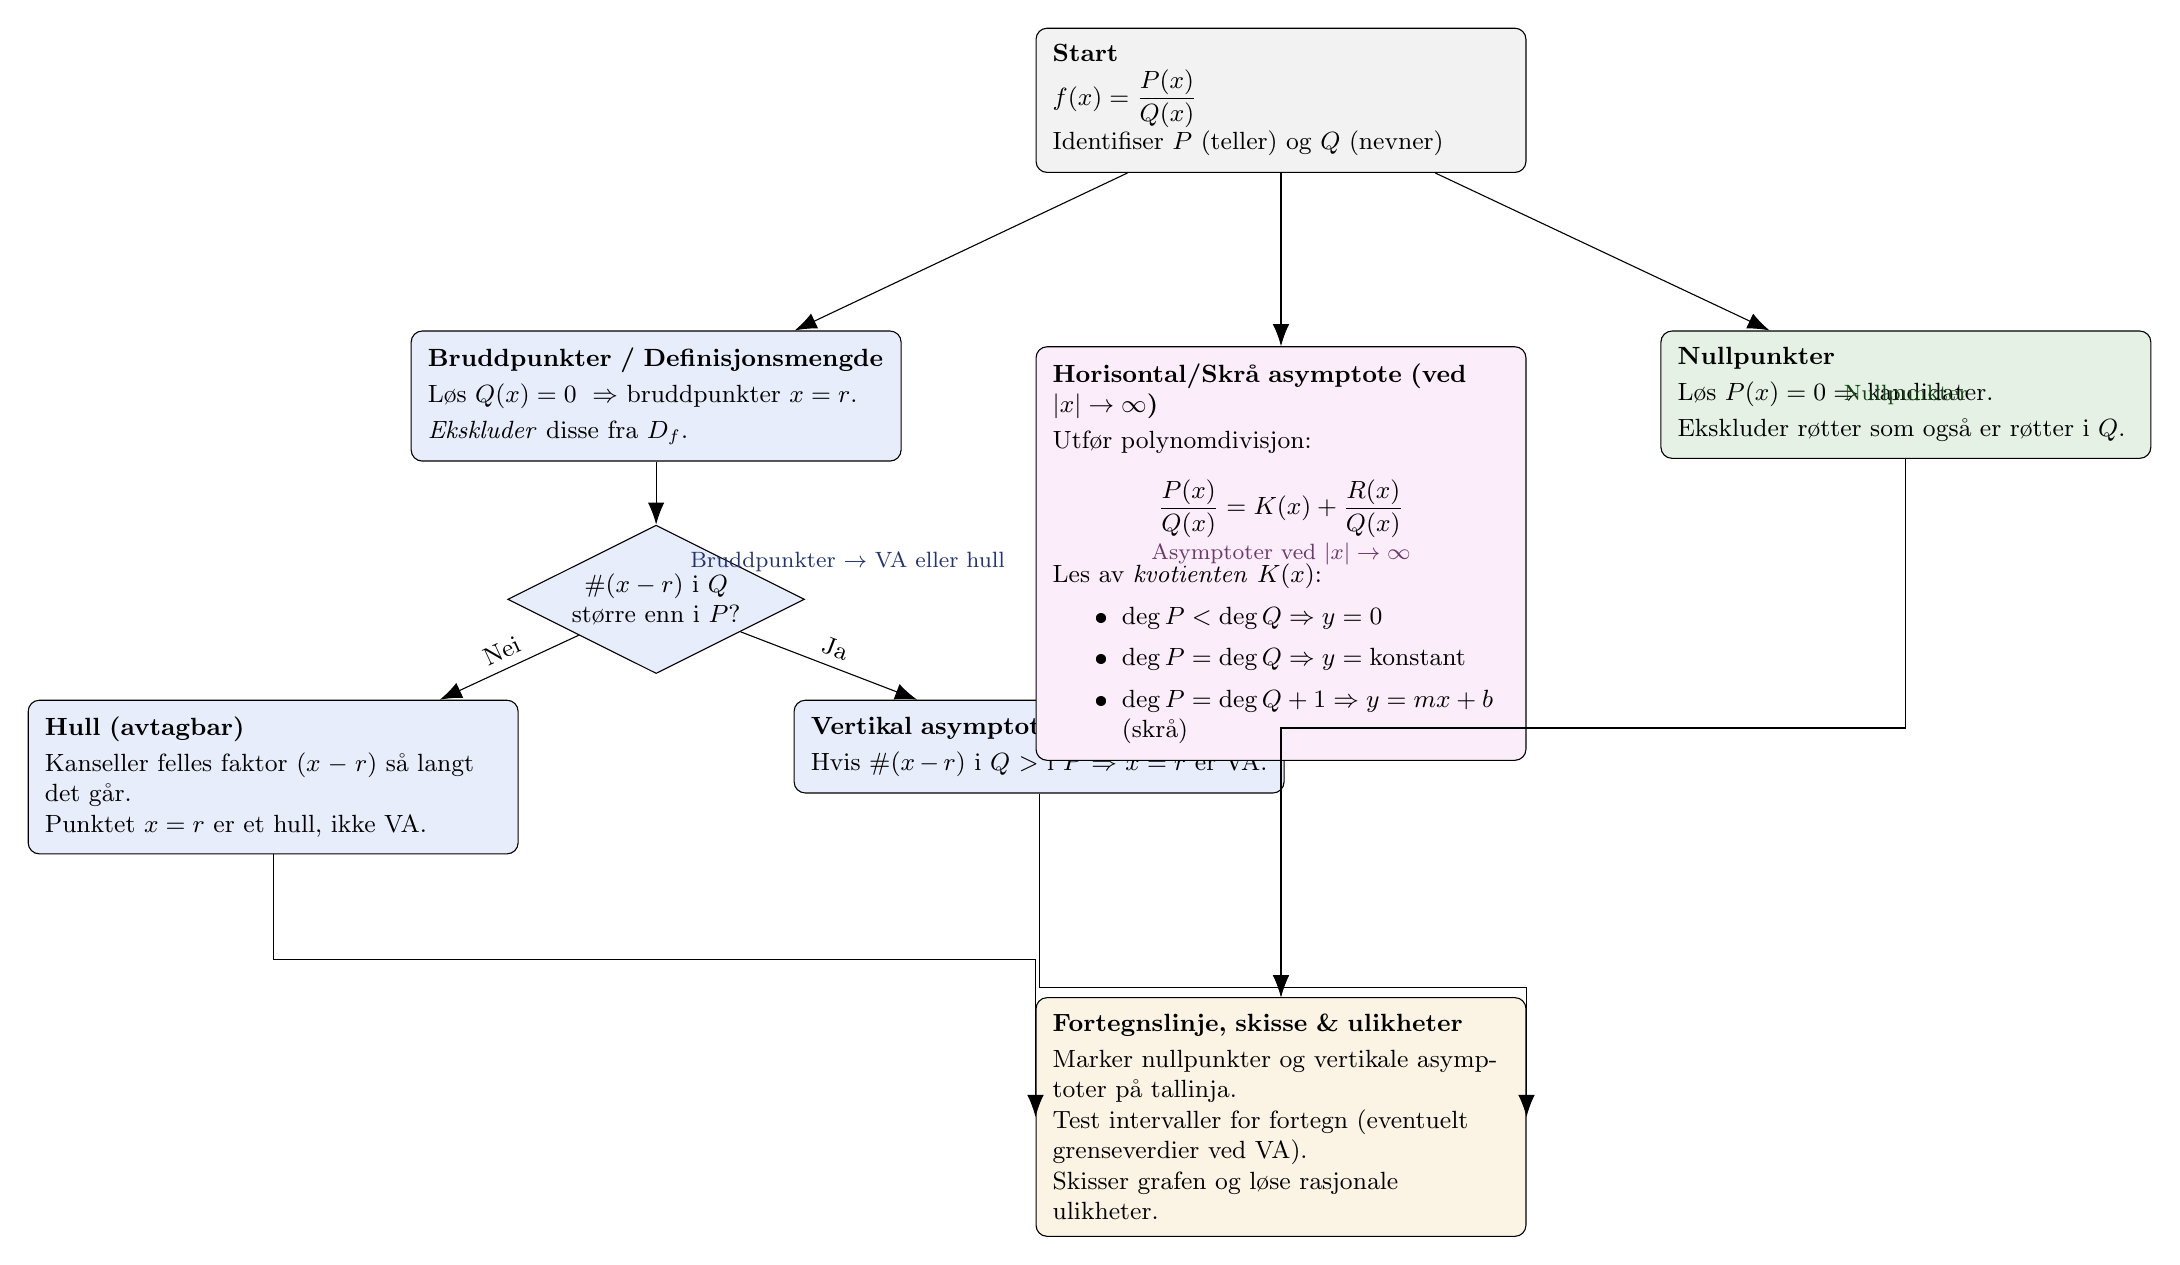
\begin{tikzpicture}[
  >={Latex[length=2.8mm]},
  font=\small,
  node distance=10mm and 12mm,
  % global box width
  box/.style = {
    draw, rounded corners,
    align=left,
    inner sep=6pt,
    minimum width=\boxw,
    text width=\boxw,
    fill=black!3
  },
  decision/.style = {
    draw, diamond, aspect=2,
    inner sep=1.5pt,
    align=center,
    fill=black!3
  },
  label/.style = {font=\small, align=center}
]

% ---- constants ----
\def\boxw{58mm}

% ---- nodes ----
% Top: input
\node[box, fill=Gray!10] (start) {\textbf{Start} \\[2pt]
$f(x)=\dfrac{P(x)}{Q(x)}$ \\
Identifiser $P$ (teller) og $Q$ (nevner)
};

% Left track: bruddpunkter → (hull vs VA)
\node[box, fill=RoyalBlue!12, below left=20mm and 17mm of start] (bp) {\textbf{Bruddpunkter / Definisjonsmengde} \\[2pt]
Løs $Q(x)=0 \ \Rightarrow$ bruddpunkter $x=r$. \\[2pt]
\emph{Ekskluder} disse fra $D_f$.
};

\node[decision, fill=RoyalBlue!12, below=8mm of bp] (dec) {$\#(x-r)$ i $Q$\\større enn i $P$?};

\node[box, fill=RoyalBlue!12, below left=8mm and 8mm of dec] (hole) {\textbf{Hull (avtagbar)} \\[2pt]
Kanseller felles faktor $(x-r)$ så langt det går.\\
Punktet $x=r$ er et hull, ikke VA.
};

\node[box, fill=RoyalBlue!12, below right=8mm and 8mm of dec] (va) {\textbf{Vertikal asymptote} \\[2pt]
Hvis $\#(x-r)$ i $Q$ $>$ i $P$ $\Rightarrow$ $x=r$ er VA.
};

% Right track: nullpunkter
\node[box, fill=ForestGreen!12, below right=20mm and 17mm of start] (zeros) {\textbf{Nullpunkter} \\[2pt]
Løs $P(x)=0 \Rightarrow$ kandidater. \\[2pt]
Ekskluder røtter som også er røtter i $Q$.
};

% Middle-lower track: asymptoter ved uendelig (polynomdivisjon)
\node[box, fill=Orchid!12, below=22mm of start] (div) {\textbf{Horisontal/Skrå asymptote (ved $|x|\to\infty$)} \\[2pt]
Utfør polynomdivisjon:
\[
\frac{P(x)}{Q(x)}=K(x)+\frac{R(x)}{Q(x)}
\]
Les av \emph{kvotienten} $K(x)$:
\begin{itemize}\setlength\itemsep{2pt}
\item $\deg P < \deg Q \Rightarrow y=0$
\item $\deg P = \deg Q \Rightarrow y=\text{konstant}$
\item $\deg P = \deg Q + 1 \Rightarrow y = mx+b$ (skrå)
\end{itemize}
};

% Final box: sign chart & sketch
\node[box, fill=Goldenrod!12, below=30mm of div] (sketch) {\textbf{Fortegnslinje, skisse \& ulikheter} \\[2pt]
Marker nullpunkter og vertikale asymptoter på tallinja.\\
Test intervaller for fortegn (eventuelt grenseverdier ved VA).\\
Skisser grafen og løse rasjonale ulikheter.
};

% ---- arrows ----
\draw[->] (start) -- (bp);
\draw[->] (start) -- (zeros);
\draw[->] (start) -- (div);

\draw[->] (bp) -- (dec);
\draw[->] (dec) -- node[label,sloped,above]{Nei} (hole);
\draw[->] (dec) -- node[label,sloped,above]{Ja} (va);

% feed into final box
\draw[->] (div) -- (sketch);
\draw[->] (zeros.south) |- ($(zeros.south)!0.5!(sketch.north)$) -| (sketch.north);
\draw[->] (hole.south) |- ($(hole.south)!0.4!(sketch.west)$) -| (sketch.west);
\draw[->] (va.south)   |- ($(va.south)!0.6!(sketch.east)$)   -| (sketch.east);

% optional titles on side tracks
\node[font=\footnotesize, RoyalBlue!50!black] at ($(bp.north)!0.5!(va.south)$) {Bruddpunkter $\to$ VA eller hull};
\node[font=\footnotesize, ForestGreen!50!black] at ($(zeros.north)!0.5!(zeros.south)$) {Nullpunkter};
\node[font=\footnotesize, Orchid!50!black] at ($(div.north)!0.5!(div.south)$) {Asymptoter ved $\lvert x\rvert\to\infty$};

\end{tikzpicture}
\end{document}